\documentclass{standalone}
\usepackage{pgfplots}
\pgfplotsset{compat=1.15}
\usepackage{mathrsfs}
\usetikzlibrary{arrows, calc}
\newcommand{\degre}{\ensuremath{^\circ}}
\pagestyle{empty}
\begin{document}
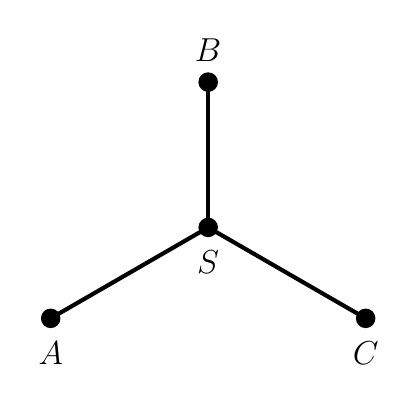
\begin{tikzpicture}[line cap=round,line join=round, scale=2]
    \begin{large}
        \draw(-1,0) node[circle,draw, fill=black, scale=0.6] (A) [label={[yshift=-0.85cm]$A$}] {};
        \draw (0, 1.5) node[circle,draw, fill=black, scale=0.6] (B) [label={[yshift=0]$B$}] {};
        \draw (1, 0) node[circle,draw, fill=black, scale=0.6] (C) [label={[yshift=-0.85cm]$C$}] {};


        % Steiner points
        \draw (0, 0.5773502691896257) node[circle,draw=black, fill=black, scale=0.6] (S) [label={[yshift=-0.85cm]$S$}] {};

        % Edges
        \foreach \source/\target in {A/S, B/S, C/S} {
                \draw[black, line width=1.5pt] (\source) -- (\target);
            }
    \end{large}
\end{tikzpicture}
\end{document}